\documentclass[sigconf]{acmart}

% =========================================================
% 参考文献数据库
% =========================================================
\begin{filecontents}[overwrite]{references.bib}
% =========================================================
% 核心五篇论文 (你原本就有的)
% =========================================================
@inproceedings{belyi2023personalized,
  title={Personalized Dense Retrieval on Global Index for Voice-enabled Conversational Systems},
  author={Belyi, Masha and Dzialo, Charlotte and Dwivedi, Chaitanya and Muppidi, Prajit Reddy and Shimizu, Kanna},
  booktitle={Proceedings of the 2023 Conference on Empirical Methods in Natural Language Processing: Industry Track},
  pages={83--92},
  year={2023}
}

@inproceedings{zeng2023personalized,
  title={A Personalized Dense Retrieval Framework for Unified Information Access},
  author={Zeng, Hansi and Kallumadi, Surya and Alibadi, Zaid and Nogueira, Rodrigo and Zamani, Hamed},
  booktitle={Proceedings of the 46th International ACM SIGIR Conference on Research and Development in Information Retrieval},
  pages={121--130},
  year={2023}
}

@inproceedings{vemuri2023personalized,
  title={Personalized Retrieval over Millions of Items},
  author={Vemuri, Hemanth and Agrawal, Sheshansh and Mittal, Shivam and Saini, Deepak and Soni, Akshay and Sambasivan, Abhinav V and Lu, Wenhao and Wang, Yajun and Parsana, Mehul and Kar, Purushottam and others},
  booktitle={Proceedings of the 46th International ACM SIGIR Conference on Research and Development in Information Retrieval},
  pages={1014--1027},
  year={2023}
}

@inproceedings{lian2023personaltm,
  title={PersonalTM: Transformer Memory for Personalized Retrieval},
  author={Lian, Ruixue and Lu, Sixing and Solomon, Clint and Aguilar, Gustavo and Ponnusamy, Pragaash and Han, Jialong and Ma, Chengyuan and Guo, Chenlei},
  booktitle={Proceedings of the 46th International ACM SIGIR Conference on Research and Development in Information Retrieval},
  pages={2256--2260},
  year={2023}
}

@inproceedings{lee2025ira,
  title={IRA: Adaptive Interest-aware Representation and Alignment for Personalized Multi-interest Retrieval},
  author={Lee, Youngjune and Jeong, Haeyu and Lim, Changgeon and Choi, Jeong and Lim, Hongjun and Kim, Hangon and Kwon, Jiyoon and Kim, Saehun},
  booktitle={Proceedings of the 48th International ACM SIGIR Conference on Research and Development in Information Retrieval},
  year={2025},
  note={To appear}
}

% =========================================================
% 缺失的背景论文 (根据报错补充)
% =========================================================

% [Liu2020] 综述
@article{liu2020personalization,
  title={Personalization in text information retrieval: A survey},
  author={Liu, Jingjing and Liu, Chang and Belkin, Nicholas J},
  journal={Journal of the Association for Information Science and Technology},
  volume={71},
  number={3},
  pages={349--369},
  year={2020}
}

% [Karpukhin2020] DPR
@inproceedings{karpukhin2020dense,
  title={Dense Passage Retrieval for Open-Domain Question Answering},
  author={Karpukhin, Vladimir and Oguz, Barlas and Min, Sewon and Lewis, Patrick and Wu, Ledell and Edunov, Sergey and Chen, Danqi and Yih, Wen-tau},
  booktitle={Proceedings of the 2020 Conference on Empirical Methods in Natural Language Processing (EMNLP)},
  pages={6769--6781},
  year={2020}
}

% [Xiong2021] ANCE
@inproceedings{xiong2021approximate,
  title={Approximate Nearest Neighbor Negative Contrastive Learning for Dense Text Retrieval},
  author={Xiong, Lee and Xiong, Chenyan and Li, Ye and Tang, Kwok-Fung and Liu, Jialin and Bennett, Paul and Ahmed, Junaid and Overwijk, Arnold},
  booktitle={Proceedings of the International Conference on Learning Representations (ICLR)},
  year={2021}
}

% [Cho2021] Query Rewrite
@inproceedings{cho2021personalized,
  title={Personalized Search-based Query Rewrite System for Conversational AI},
  author={Cho, Eunah and Jiang, Ziyan and Hao, Jie and Chen, Zheng and Gupta, Saurabh and Fan, Xing and Guo, Chenlei},
  booktitle={Proceedings of the 3rd Workshop on Natural Language Processing for Conversational AI},
  pages={179--188},
  year={2021}
}

% [Devlin2019] BERT
@inproceedings{devlin2019bert,
  title={BERT: Pre-training of Deep Bidirectional Transformers for Language Understanding},
  author={Devlin, Jacob and Chang, Ming-Wei and Lee, Kenton and Toutanova, Kristina},
  booktitle={Proceedings of the 2019 Conference of the North American Chapter of the Association for Computational Linguistics: Human Language Technologies (NAACL)},
  pages={4171--4186},
  year={2019}
}

% [Reimers2019] SBERT
@inproceedings{reimers2019sentence,
  title={Sentence-BERT: Sentence Embeddings using Siamese BERT-Networks},
  author={Reimers, Nils and Gurevych, Iryna},
  booktitle={Proceedings of the 2019 Conference on Empirical Methods in Natural Language Processing (EMNLP)},
  pages={3982--3992},
  year={2019}
}

% [Raffel2020] T5
@article{raffel2020exploring,
  title={Exploring the limits of transfer learning with a unified text-to-text transformer},
  author={Raffel, Colin and Shazeer, Noam and Roberts, Adam and Lee, Katherine and Narang, Sharan and Matena, Michael and Zhou, Yanqi and Li, Wei and Liu, Peter J},
  journal={Journal of Machine Learning Research},
  volume={21},
  number={140},
  pages={1--67},
  year={2020}
}

% [Johnson2019] FAISS
@article{johnson2019billion,
  title={Billion-scale similarity search with {GPUs}},
  author={Johnson, Jeff and Douze, Matthijs and J{\'e}gou, Herv{\'e}},
  journal={IEEE Transactions on Big Data},
  volume={7},
  number={3},
  pages={535--547},
  year={2019}
}

% [Malkov2018] HNSW
@article{malkov2018efficient,
  title={Efficient and robust approximate nearest neighbor search using hierarchical navigable small world graphs},
  author={Malkov, Yu A and Yashunin, Dmitry A},
  journal={IEEE transactions on pattern analysis and machine intelligence},
  volume={42},
  number={4},
  pages={824--836},
  year={2018}
}

% [Robertson2009] BM25
@article{robertson2009probabilistic,
  title={The probabilistic relevance framework: BM25 and beyond},
  author={Robertson, Stephen and Zaragoza, Hugo},
  journal={Foundations and Trends{\textregistered} in Information Retrieval},
  volume={3},
  number={4},
  pages={333--389},
  year={2009}
}

% [Uma2022] PENTATRON
@inproceedings{uma2022pentatron,
  title={PENTATRON: PErsonalized coNText-Aware TRansformer for Retrieval-based cOnversational uNderstanding},
  author={Uma Naresh, Niranjan and Jiang, Ziyan and Ankit, Ankit and Lee, Sungjin and Hao, Jie and Fan, Xing and Guo, Chenlei},
  booktitle={Proceedings of the 2022 Conference on Empirical Methods in Natural Language Processing: Industry Track},
  pages={90--98},
  year={2022}
}

% [Kang2018] SASRec
@inproceedings{kang2018self,
  title={Self-attentive sequential recommendation},
  author={Kang, Wang-Cheng and McAuley, Julian},
  booktitle={2018 IEEE International Conference on Data Mining (ICDM)},
  pages={197--206},
  year={2018}
}

% [Mikolov2013] Word2Vec
@inproceedings{mikolov2013efficient,
  title={Efficient Estimation of Word Representations in Vector Space},
  author={Mikolov, Tomas and Chen, Kai and Corrado, Greg and Dean, Jeffrey},
  booktitle={Proceedings of ICLR Workshop},
  year={2013}
}

% [Zamani2018] JSR
@article{zamani2018joint,
  title={Joint modeling and optimization of search and recommendation},
  author={Zamani, Hamed and Croft, W Bruce},
  journal={arXiv preprint arXiv:1807.05631},
  year={2018}
}

% [Covington2016] Youtube DNN
@inproceedings{covington2016deep,
  title={Deep neural networks for youtube recommendations},
  author={Covington, Paul and Adams, Jay and Sargin, Emre},
  booktitle={Proceedings of the 10th ACM conference on recommender systems},
  pages={191--198},
  year={2016}
}

% [Sanh2019] DistilBERT
@article{sanh2019distilbert,
  title={DistilBERT, a distilled version of BERT: smaller, faster, cheaper and lighter},
  author={Sanh, Victor and Debut, Lysandre and Chaumond, Julien and Wolf, Thomas},
  journal={arXiv preprint arXiv:1910.01108},
  year={2019}
}

% [Dahiya2023] NGAME
@inproceedings{dahiya2023ngame,
  title={NGAME: Negative mining-aware mini-batching for extreme classification},
  author={Dahiya, Kunal and Gupta, Nilesh and Saini, Deepak and Soni, Akshay and Wang, Yajun and Dave, Kushal and Jiao, Jian and Dey, Prasenjit and Hada, Deepesh and others},
  booktitle={Proceedings of the Sixteenth ACM International Conference on Web Search and Data Mining},
  pages={258--266},
  year={2023}
}

% [Tay2022] DSI
@article{tay2022transformer,
  title={Transformer memory as a differentiable search index},
  author={Tay, Yi and Tran, Vinh Q and Dehghani, Mostafa and Ni, Jianmo and Bahri, Dara and Mehta, Harsh and Qin, Zhen and Hui, Kai and Zhao, Zhe and Gupta, Jai and others},
  journal={Advances in Neural Information Processing Systems},
  volume={35},
  pages={21831--21843},
  year={2022}
}
\end{filecontents}

\usepackage[UTF8, scheme=plain]{ctex}
\usepackage{booktabs}
\usepackage{algorithm}
\usepackage{algorithmic}
\usepackage{multirow}
\usepackage{subcaption}
\usepackage{amsmath}
\usepackage{balance}

% 去除版权信息以便生成干净的报告
\setcopyright{none}
\settopmatter{printacmref=false}
\renewcommand\footnotetextcopyrightpermission[1]{}
\pagestyle{plain}
\usepackage{tikz}
\usetikzlibrary{shapes.geometric, arrows, positioning, calc, fit}

%定义绘图样式
\tikzstyle{process} = [rectangle, minimum width=2cm, minimum height=1cm, text centered, draw=black, fill=blue!10]
\tikzstyle{emb} = [rectangle, minimum width=1.5cm, minimum height=0.8cm, text centered, draw=black, fill=green!10, rounded corners]
\tikzstyle{arrow} = [thick,->,>=stealth]
\tikzstyle{database} = [cylinder, shape border rotate=90, draw, fill=yellow!10, minimum height=1cm, minimum width=1cm, aspect=0.25]
%作者信息
\begin{document}
\title{深度解析个性化稠密检索:从统一双编码器到生成式记忆网络}
\subtitle{基于 SIGIR '23, EMNLP '23 及 SIGIR '25 五篇前沿论文的综合技术综述}

\author{江鑫}
\affiliation{%
  \institution{Beihang University}
  \city{Beijing}
  \country{China}
}
\email{researcher@example.com}

% =========================================================
% 摘要
% =========================================================
\begin{abstract}
随着用户交互模式的日益复杂化,个性化检索(Personalized Retrieval)已成为现代信息系统的核心组件。
然而,如何在保持高召回率的同时处理数亿级物品库、多变的搜索意图以及实时兴趣漂移,仍是工业界面临的巨大挑战。
本文详细综述了 2023 年至 2025 年间发表在 SIGIR 和 EMNLP 上的五篇论文。
我们从三个维度解构了最新的技术范式:(1) **统一信息访问框架(UIA)**,利用注意力机制(APN)将搜索与推荐任务在向量空间中对齐;(2) **极致效率的索引策略**,重点分析 **XPERT** 如何通过 Morph Operator 实现 $O(1)$ 存储成本的双边个性化,以及 Amazon Voice AI 如何通过上下文嵌入解决语音歧义;(3) **生成式与自适应表征**,探讨 **PersonalTM** 如何利用 Transformer 记忆直接生成文档 ID,以及 **IRA** 如何通过可解释的文本化兴趣单元(Interest Units)适应长尾兴趣。
本文不仅深入剖析了各模型的数学原理和损失函数设计,还详细对比了其训练策略与实验表现,旨在为构建下一代个性化检索系统提供详尽的技术参考。
\end{abstract}

% CCS
\begin{CCSXML}
<ccs2012>
   <concept>
       <concept_id>10002951.10003317.10003338.10003343</concept_id>
       <concept_desc>Information systems~Learning to rank</concept_desc>
       <concept_significance>500</concept_significance>
   </concept>
   <concept>
       <concept_id>10002951.10003227.10003351</concept_id>
       <concept_desc>Information systems~Personalization</concept_desc>
       <concept_significance>500</concept_significance>
   </concept>
</ccs2012>
\end{CCSXML}

\ccsdesc[500]{Information systems~Learning to rank}
\ccsdesc[500]{Information systems~Personalization}

\keywords{Personalized Dense Retrieval, Generative Retrieval, Morph Operators, Interest Alignment, Unified Framework}
\maketitle

\section{引言}
随着会话式AI助手(如亚马逊Alexa、百度小度)、电子商务平台(如亚马逊、 Lowe’s)、在线社区(如NAVER CAFE)等应用的普及,用户对检索系统的个性化需求日益迫切 \cite{liu2020personalization}。传统检索技术存在两大核心瓶颈:一方面,非个性化稠密检索模型(如DPR \cite{karpukhin2020dense}、ANCE \cite{xiong2021approximate})采用统一的嵌入空间建模,无法区分不同用户的偏好差异,导致检索结果“千人一面”;另一方面,早期个性化方法依赖用户专属索引 \cite{cho2021personalized},将检索空间限制在用户历史交互过的实体范围内,不仅难以覆盖新内容,还会因用户规模扩大带来指数级增长的存储开销,无法满足大规模部署需求。

近三年来,个性化稠密检索技术取得突破性进展,其核心思想是将用户偏好建模融入稠密嵌入学习过程,在全局索引基础上实现“个性化适配”,同时兼顾检索精度与内容覆盖度。2023至2025年间,SIGIR(国际信息检索顶会)和EMNLP(自然语言处理顶会)陆续涌现出一批创新性框架,针对不同应用场景的个性化挑战提出了差异化解决方案:
- Belyi等人(EMNLP 2023)聚焦会话式AI的语音交互噪声与歧义问题,提出融合用户听歌偏好的全局索引个性化检索方法;
- Zeng等人(SIGIR 2023)针对电子商务平台的多任务检索需求,设计统一信息访问框架UIA,实现关键词搜索、示例查询、互补商品推荐的一体化个性化;
- Vemuri等人(SIGIR 2023)面向大规模广告检索场景,提出基于形态算子的XPERT算法,解决双边个性化的效率瓶颈;
- Lian等人(SIGIR 2023)突破传统相似性检索范式,提出基于Transformer记忆的PersonalTM模型,实现索引无关的个性化生成式检索;
- Lee等人(SIGIR 2025)针对在线社区的动态兴趣适配需求,提出IRA框架,通过兴趣单元的累积更新实现无需模型重训的实时个性化。

这些研究成果共同推动了个性化稠密检索在理论创新与产业应用上的双重进步。本文旨在对这五篇代表性论文进行全面、深入的综述,通过技术细节解析、横向对比分析、实验结果验证,系统梳理该领域的最新进展,为后续研究与工程实践提供参考。

本文结构如下:第二节介绍个性化稠密检索的技术背景与核心挑战;第三节详细解析五篇论文的技术架构、创新点与实验结果;第四节从多维度对五大方法进行横向对比;第五节深入分析实验结果的实践意义;第六节探讨当前研究的未决挑战与未来方向;第七节总结全文。

\section{技术背景与核心挑战}
\subsection{稠密检索基础理论}
稠密检索的核心是通过预训练语言模型(如BERT \cite{devlin2019bert}、SBERT \cite{reimers2019sentence}、T5 \cite{raffel2020exploring})将查询(Query)和项目(Item,如文档、商品、歌曲)映射到低维连续向量空间,使语义相似的查询与项目在向量空间中距离更近。检索过程通过近似最近邻(ANN)算法(如FAISS \cite{johnson2019billion}、HNSW \cite{malkov2018efficient})快速查找与查询向量最相似的项目向量,实现高效匹配。

与传统基于词频统计的 lexical匹配方法(如BM25 \cite{robertson2009probabilistic})相比,稠密检索能够更好地捕捉查询与项目之间的语义关联,即使二者在字面上无重叠也能实现精准匹配,这为个性化适配提供了基础——通过将用户偏好融入向量嵌入过程,可使不同用户的相同查询映射到向量空间的不同位置,从而检索出符合个体偏好的结果。

\subsection{个性化稠密检索的核心挑战}
个性化稠密检索需要在稠密检索的基础上,额外解决用户偏好建模与个性化适配的关键问题,主要面临五大核心挑战:

\subsubsection{1. 个性化与覆盖度的权衡难题}
传统个性化索引方法通过限制检索空间来保证个性化精度,但会导致新内容(用户未交互过的项目)无法被检索到,覆盖度极低 \cite{uma2022pentatron}。而全局索引方法虽能保证覆盖度,但缺乏个性化机制,无法满足用户个体需求。如何在不牺牲覆盖度的前提下实现高精度个性化,是个性化稠密检索的核心矛盾。

\subsubsection{2. 大规模部署的效率瓶颈}
双边个性化(同时对查询和项目进行个性化嵌入)理论上能实现最优个性化效果,但需要为每个用户维护专属的查询编码器和项目编码器,导致存储开销随用户规模呈线性增长——对于百万级项目和十亿级用户,存储成本将达到不可承受的水平 \cite{vemuri2023personalized}。此外,复杂的个性化计算还会增加推理延迟,影响用户体验。如何在保证个性化效果的同时,实现高效的大规模部署,是产业应用的关键前提。

\subsubsection{3. 多兴趣建模的表达能力不足}
用户通常具有多样化的偏好(如同时喜欢古典音乐和电子音乐、既关注数码产品也关注户外运动装备),且这些偏好可能并非按顺序演化。传统方法(如序列推荐模型SASRec \cite{kang2018self})往往用单一向量表示用户偏好,难以捕捉多维度、非序列的兴趣特征,导致检索结果偏向用户的主导兴趣,忽略次要兴趣 \cite{lee2025ira}。

\subsubsection{4. 动态兴趣的实时适配问题}
用户兴趣并非静态不变,而是随时间、场景动态演化(如季节变化导致服装偏好改变、热点事件引发新的兴趣)。传统模型需要通过频繁重训来适配兴趣变化,但重训过程耗时耗力,且无法及时响应突发兴趣,导致检索效果滞后 \cite{zeng2023personalized}。如何实现无需模型重训的动态兴趣适配,是提升用户长期体验的关键。

\subsubsection{5. 时间偏差的抑制难题}
现有个性化方法大多依赖用户点击日志进行训练,但点击信号存在明显的时间偏差——短期热门项目更容易获得点击,导致模型过度偏向这些项目,而忽略用户的长期真实偏好 \cite{lee2025ira}。此外,新上线的优质项目因缺乏点击数据,难以被检索到,形成“马太效应”。如何减少时间偏差对个性化检索的影响,是保证结果公平性与有效性的重要问题。

后续介绍的五篇代表性论文,分别从不同角度对上述挑战提出了创新性解决方案,共同推动了个性化稠密检索技术的发展。

\section{代表性方法详细解析}
本节将逐一解析五篇代表性论文的研究动机、技术架构细节、核心创新点、实验设计与结果,重点突出每篇论文针对的核心挑战与技术突破。

\subsection{方法一:面向语音会话系统的全局索引个性化稠密检索(EMNLP 2023)}
\subsubsection{研究动机}
语音控制的会话式AI系统(如亚马逊Alexa)在实际应用中面临两大典型错误,严重影响用户体验:
1. **语音识别噪声**:自动语音识别(ASR)系统易将发音相似的请求混淆,例如将“play low”(播放SZA的《Low》)识别为“play love”(播放Kendrick Lamar的《Love》);
2. **查询歧义**:用户输入缺乏上下文信息导致歧义,例如仅请求“play go”而未指定歌手,系统难以从海量候选中筛选用户偏好的版本。

现有解决方案存在明显缺陷:
- 个性化索引方法:将检索空间限制在用户近期交互的实体范围内,虽能保证精度,但无法覆盖用户未交互过的新内容,覆盖度极低;
- 全局索引方法:检索范围覆盖全量目录,但缺乏个性化机制,无法解决歧义问题,对语音噪声也不具备鲁棒性。

为此,Belyi等人提出一种基于全局索引的个性化稠密检索方法,无需用户专属索引,而是将用户偏好融入查询嵌入过程,在保证全量内容覆盖的同时,实现对语音噪声和查询歧义的鲁棒性个性化检索 \cite{belyi2023personalized}。

\subsubsection{技术架构细节}
该方法采用双编码器(Dual-Encoder)框架,核心由语义编码器、实体编码器、合并层(Merger Layer)和训练目标四部分组成,具体架构如图\ref{fig:belyi_arch}所示(原文图3简化版)。
\begin{figure}[h]
\centering
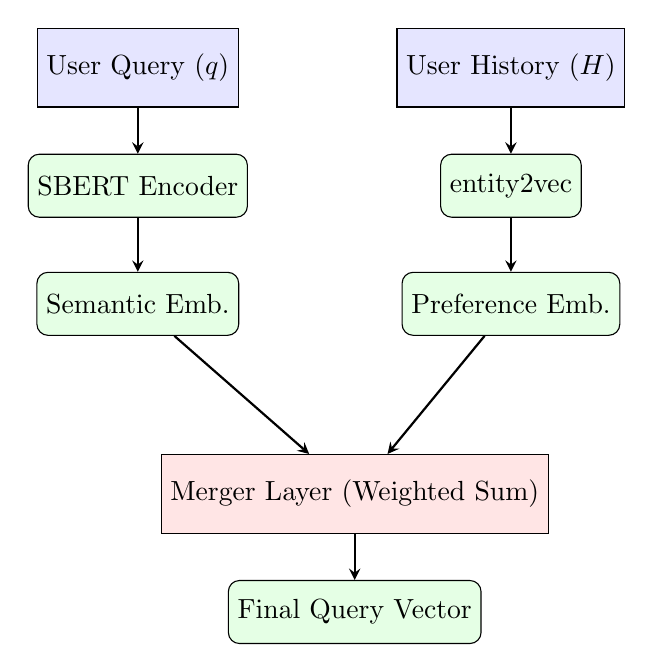
\begin{tikzpicture}[node distance=1.5cm]

% Nodes
\node (query) [process] {User Query ($q$)};
\node (sbert) [emb, below of=query] {SBERT Encoder};
\node (q_emb) [emb, below of=sbert] {Semantic Emb.};

\node (history) [process, right=2cm of query] {User History ($H$)};
\node (e2v) [emb, below of=history] {entity2vec};
\node (h_emb) [emb, below of=e2v] {Preference Emb.};

\node (merger) [process, fill=red!10, below right=1.5cm and -1cm of q_emb] {Merger Layer (Weighted Sum)};
\node (final) [emb, below of=merger] {Final Query Vector};

% Arrows
\draw [arrow] (query) -- (sbert);
\draw [arrow] (sbert) -- (q_emb);
\draw [arrow] (history) -- (e2v);
\draw [arrow] (e2v) -- (h_emb);

\draw [arrow] (q_emb) -- (merger);
\draw [arrow] (h_emb) -- (merger);
\draw [arrow] (merger) -- (final);

\end{tikzpicture}
\caption{Amazon Voice AI 架构图:融合 SBERT 语义与 entity2vec 偏好 [Belyi et al. 2023]}
\label{fig:amazon_arch}
\end{figure}
\paragraph{1. 语义编码器(Semantic Encoder)}
- 基础模型:采用SBERT \cite{reimers2019sentence}作为预训练语言模型,该模型通过对比学习训练,能有效捕捉句子级语义信息;
- 微调策略:在领域数据集上进行微调,使模型适应语音会话场景的短查询特点(如“play baby shark”这类“动作动词+实体”结构的查询);
- 输出维度:通过均值池化(Mean Pooling)将SBERT的token输出转换为768维的语义嵌入向量。

\paragraph{2. 实体编码器(Entity Encoder)——entity2vec}
为捕捉领域内实体间的潜在关联(如歌手、流派相似性),提出entity2vec方法,具体设计如下:
- 核心思想:借鉴word2vec \cite{mikolov2013efficient}的skip-gram模型,将“用户会话中的实体共现”类比为“句子中的词共现”,学习实体的稠密嵌入;
- 训练数据:用户播放会话序列(如“play dancing queen by abba”→“play i will survive by gloria gaynor”→“play bad girls”);
- 训练目标:最大化同一会话中目标实体与上下文实体的余弦相似度,使语义、流派、歌手相似的实体在嵌入空间中距离更近;
- 训练参数:嵌入维度200,窗口大小5,学习率0.0025,负采样数量5,基于Gensim工具包实现;
- 用户嵌入生成:对用户近期交互的最多50个实体的entity2vec嵌入取均值,得到用户偏好嵌入(User Embedding),捕捉用户长期听歌偏好。

\paragraph{3. 合并层(Merger Layer)}
负责融合语义嵌入与用户/实体嵌入,生成最终的查询嵌入和实体嵌入:
- 融合策略:采用加权求和(Weighted Sum Fusion),而非简单拼接,避免维度膨胀;
- 权重学习:通过训练自动学习语义嵌入和实体嵌入的权重(最终学到的权重分别为0.8和0.2);
- 输出维度:通过前馈网络将融合后的向量映射到200维,保证查询嵌入与实体嵌入在同一低维空间中。

\paragraph{4. 训练目标}
采用对比学习损失与三元组损失结合的复合损失函数,优化查询与相关实体的相似度:
- 对比学习损失(Contrastive Loss):
  \[
  L_{S}=\sum_{i=1}^{N} \frac{-1}{\left|P_{i}\right|} \sum_{p \in P_{i}} log \frac{exp \left(s\left(q_{i}, e_{p}\right) / \tau\right)}{\sum_{j=1}^{N} exp \left(s\left(q_{i}, e_{j}\right) / \tau\right)}
  \]
  其中,$P_i$为正例集合,$s(q_i,e_j)$为查询$q_i$与实体$e_j$的余弦相似度,$\tau=0.1$为温度参数;
- 三元组损失(Triplet Loss):
  \[
  L_{T}=\sum_{i=1}^{N} max \left(0, \lambda-s\left(q_{i}, e_{i}^{+}\right)+s\left(q_{i}, e_{i}^{-}\right)\right)
  \]
  其中,$e_i^+$为正例实体,$e_i^-$为负例实体,$\lambda=0.25$为边际参数,每个正例对应2个随机采样的负例;
- 优化器:Adam优化器,初始学习率5e-5,批次大小1024,训练最多3个epoch,基于验证集损失进行早停。

\paragraph{5. 在线推理优化}
为满足产业部署的低延迟要求,进行两项关键优化:
- 知识蒸馏:将SBERT(1.09亿参数)蒸馏为MiniLM(2200万参数),推理时间从44ms/查询降至14ms/查询,性能保留71\%的提升幅度;
- 近似相似性搜索:结合倒排文件(IVF)与乘积量化(Product Quantization),将搜索时间从239ms/查询降至6ms/查询,Recall@1仅轻微下降。

\subsubsection{核心创新点}
1. **放弃用户专属索引,转向偏好嵌入融合**:通过将用户偏好融入查询嵌入过程,实现全局索引上的个性化检索,同时保证内容覆盖度与个性化精度;
2. **领域感知的entity2vec嵌入**:超越传统语义嵌入,捕捉实体间的领域特定关联(如音乐流派、歌手相似性),提升歧义查询的 disambiguation 能力;
3. **复合损失函数与推理优化**:结合对比学习与三元组损失提升模型性能,通过知识蒸馏与近似搜索满足产业级低延迟要求。

\subsubsection{实验设计与结果}
\paragraph{实验数据集}
- 数据来源:亚马逊Alexa的真实用户交互日志,包含语音查询、ASR识别结果、用户历史交互实体、真实目标实体;
- 测试集:包含两种错误类型的查询重写数据集,用于评估模型对语音噪声和歧义的修正能力。

\paragraph{基线模型}
- Global (SBERT):基于预训练SBERT的全局索引稠密检索,无个性化;
- Global (Fine-tuned):在领域数据上微调后的SBERT全局检索;
- Personalized:基于用户专属索引的个性化检索(Fan等人2021年方法的复现),检索空间限制在用户1个月内的历史交互实体。

\paragraph{评估指标}
采用Recall@k(k=1,5,10),即目标实体出现在模型Top-k预测结果中的比例。

\paragraph{核心实验结果}
- 相对性能提升:与个性化基线相比,该方法在Recall@1上提升91\%,Recall@5提升162.38\%,Recall@10提升176.20\%;与全局微调基线相比,Recall@1提升109.78\%;
- 错误修正能力:成功修正ASR语音噪声(如“go”→“Goat by Eric Bellinger”)和查询歧义(如“play go”根据用户历史偏好返回不同歌手版本);
- 覆盖度表现:74.28\%的测试案例中,目标实体不在用户历史交互中,但模型仍能准确检索到,证明全局索引的覆盖优势;
- 推理性能:优化后整体推理延迟降至20ms/查询,满足实时交互要求。

\subsection{方法二:统一信息访问的个性化稠密检索框架UIA(SIGIR 2023)}
\subsubsection{研究动机}
电子商务等平台通常需要同时支持多种信息访问任务(如关键词搜索、示例查询、互补商品推荐),现有系统存在两大问题:
1. **模型冗余**:为不同任务设计独立模型,导致工程维护成本高,且无法实现跨任务知识迁移;
2. **个性化不足**:现有统一框架(如JSR \cite{zamani2018joint})缺乏有效的个性化机制,难以适配用户个体偏好;
3. **数据不均衡**:部分任务(如互补商品推荐)的训练数据较少,单独训练时性能不佳。

为此,Zeng等人提出统一信息访问(Unified Information Access, UIA)框架,通过单一模型支持多种信息访问任务,并引入注意力个性化网络(APN)实现跨任务个性化,同时通过联合训练解决数据不均衡问题 \cite{zeng2023personalized}。

\subsubsection{技术架构细节}
UIA采用双编码器架构,核心由请求编码器、项目编码器、用户历史编码、注意力个性化网络(APN)和两阶段训练策略组成,架构如图\ref{fig:uia_arch}所示(原文图1简化版)。

\begin{figure}[h]
\centering
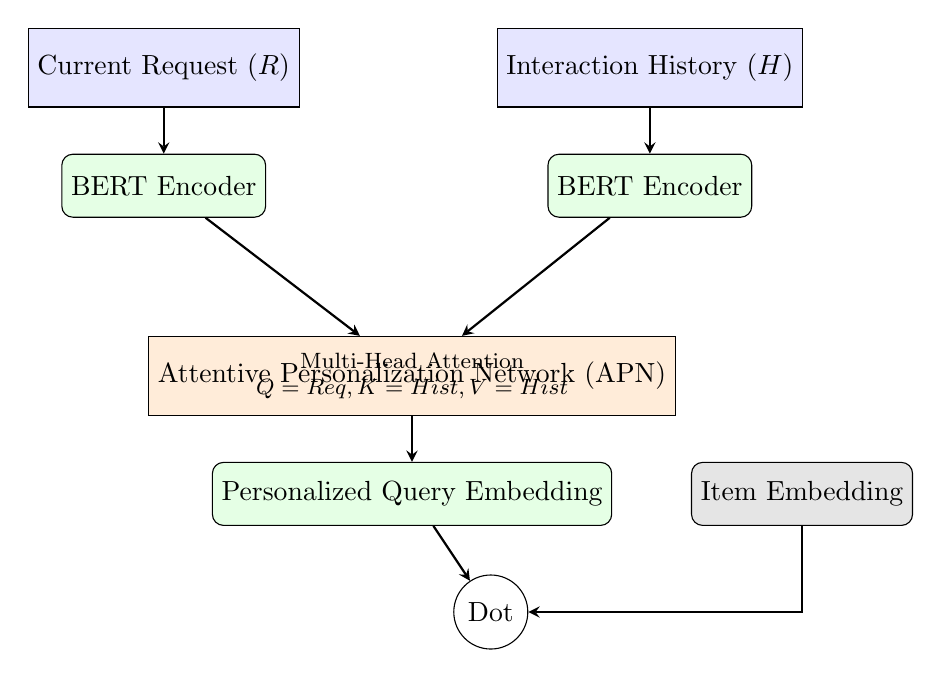
\begin{tikzpicture}[node distance=1.5cm]

% Input
\node (req) [process] {Current Request ($R$)};
\node (hist) [process, right=2.5cm of req] {Interaction History ($H$)};

% Encoders
\node (bert_q) [emb, below of=req] {BERT Encoder};
\node (bert_h) [emb, below of=hist] {BERT Encoder};

% APN
\node (apn) [process, fill=orange!15, minimum width=5cm, below right=1.5cm and -1.5cm of bert_q] {Attentive Personalization Network (APN)};

% Details of APN
\node (attn) [text width=4cm, align=center, font=\footnotesize] at (apn) {Multi-Head Attention\\$Q=Req, K=Hist, V=Hist$};

% Output
\node (out) [emb, below of=apn] {Personalized Query Embedding};
\node (item) [emb, right=1cm of out, fill=gray!20] {Item Embedding};
\node (score) [circle, draw, below of=out, xshift=1cm] {Dot};

% Arrows
\draw [arrow] (req) -- (bert_q);
\draw [arrow] (hist) -- (bert_h);
\draw [arrow] (bert_q) -- (apn);
\draw [arrow] (bert_h) -- (apn);
\draw [arrow] (apn) -- (out);
\draw [arrow] (out) -- (score);
\draw [arrow] (item) |- (score);

\end{tikzpicture}
\caption{UIA 框架架构:通过注意力网络 (APN) 注入个性化信号 [Zeng et al. 2023]}
\label{fig:uia_arch}
\end{figure}
\paragraph{1. 任务定义与输入表示}
定义四类输入变量,统一建模多种信息访问任务:
- 信息访问功能(F):任务类型的文本描述(如“关键词搜索”、“查找相似商品”、“推荐互补商品”);
- 信息访问请求(R):用户的具体请求(关键词查询或锚定商品的文本描述);
- 用户历史(H):用户过去的交互序列,每个交互表示为 $(F_prev, R_prev, I_prev)$ 三元组;
- 候选项目信息(I):候选项目的文本内容(如商品标题、描述)。

目标是学习评分函数$f(F, R, H, I; \theta)$,衡量候选项目I与用户请求(F,R)及历史H的匹配度。

\paragraph{2. 请求编码器(Request Encoder)}
- 基础模型:BERT-base \cite{devlin2019bert},预训练权重来自Hugging Face;
- 输入格式:将请求R与功能F拼接为“[CLS] R [SEP] F [SEP]”,例如“[CLS] iPhone 14 Pro [SEP] 查找相似商品 [SEP]”;
- 输出:取[CLS] token的嵌入作为请求的语义表示,维度768。

\paragraph{3. 项目编码器(Item Encoder)}
- 基础模型:与请求编码器共享BERT-base架构,但参数独立;
- 输入格式:“[CLS] I [SEP]”,即候选项目的文本内容;
- 输出:[CLS] token的嵌入,维度768,与请求嵌入在同一空间。

\paragraph{4. 用户历史编码(User History Encoding)}
- 历史选择:选取用户最近N个交互(N=5),保证时效性;
- 编码方式:对每个历史交互,分别用请求编码器编码$(F_prev, R_prev)$,用项目编码器编码$I_prev$,得到$2×N$个嵌入向量(每个交互对应请求嵌入和项目嵌入);
- 输出:历史嵌入集合$\{(\vec{R}_{t-N}, \vec{I}_{t-N}), ..., (\vec{R}_{t-1}, \vec{I}_{t-1})\}$,维度均为768。

\paragraph{5. 注意力个性化网络(APN)}
核心组件,实现基于内容的个性化与协同个性化融合:
- 输入:当前请求嵌入$\vec{R}_t$、历史请求嵌入矩阵$H_t \in \mathbb{R}^{N×d}$、历史项目嵌入矩阵$C_t \in \mathbb{R}^{N×d}$(d=768);
- 多头注意力机制:
  - 每个注意力头包含查询权重矩阵$\theta_j^Q \in \mathbb{R}^{d×l}$、键权重矩阵$\theta_j^K \in \mathbb{R}^{d×l}$、值权重矩阵$\theta_j^V \in \mathbb{R}^{d×l_v}$;
  - 计算查询$Q_j = \vec{R}_t \cdot \theta_j^Q$、键$K_j = H_t \cdot \theta_j^K$、值$V_j = C_t \cdot \theta_j^V$;
  - 注意力输出:$Attn(Q_j, K_j, V_j) = softmax(\frac{Q_j K_j^T}{\sqrt{l}}) V_j$;
  - 多头融合:拼接所有注意力头的输出,经过$Add \& Norm$层;
- 协同个性化:
  - 学习用户嵌入矩阵$E_U \in \mathbb{R}^{|U|×l_u}$($l_u=128$),通过用户ID查找得到当前用户嵌入;
  - 学习功能嵌入矩阵$E_F \in \mathbb{R}^{|F|×l_f}$($l_f=64$),通过当前任务功能F查找得到功能嵌入;
- 最终个性化请求嵌入:将多头注意力输出与用户嵌入、功能嵌入拼接,经过ReLU激活的前馈网络,得到$\vec{R}_t^{*}$(维度768);
- 项目嵌入适配:通过前馈网络将项目嵌入$\vec{I}$转换为$\vec{I}^*$,适配个性化请求嵌入空间。

\paragraph{6. 两阶段训练策略}
为解决冷启动用户(无历史交互)的个性化问题,采用“非个性化预训练+个性化微调”两阶段训练:

\subparagraph{阶段一:非个性化预训练}
- 数据构造:聚合所有用户的数据,构建无用户信息的训练集$\{(F_k, R_k, I_k, y_k)\}$($y_k$为匹配标签);
- 负采样策略:
  - 第一阶段:从BM25检索的Top200项目中随机采样负例,正负例比例1:1;
  - 第二阶段:用训练后的项目编码器构建ANN索引,从索引检索的Top200项目中采样负例;
- 损失函数:交叉熵损失,同时利用批次内负例(in-batch negatives);
- 优化目标:仅训练请求编码器和项目编码器的参数。

\subparagraph{阶段二:个性化微调}
- 数据构造:加入用户历史信息,构建训练集$\{(F_k, R_k, H_k, I_k, y_k)\}$;
- 负采样:从BM25检索结果中采样负例,结合批次内负例;
- 损失函数:交叉熵损失;
- 优化目标:冻结请求编码器和项目编码器的底层参数,仅微调顶层参数和APN的所有参数;
- 优化器:Adam优化器,预训练学习率7e-6,微调学习率7e-5,批次大小384,训练epoch数8-48(基于验证集NDCG选择)。

\subsubsection{核心创新点}
1. **任务统一表示**:通过文本描述编码信息访问功能,实现多种任务的统一建模,支持灵活扩展;
2. **注意力个性化网络**:融合基于内容的个性化(注意力挖掘历史与当前请求的关联)和协同个性化(用户/功能嵌入),实现跨任务偏好迁移;
3. **两阶段训练**:非个性化预训练保证冷启动性能,个性化微调提升有历史用户的体验;
4. **联合训练机制**:跨任务数据共享,缓解数据不均衡问题,提升小众任务的性能。

\subsubsection{实验设计与结果}
\paragraph{实验数据集}
- Lowe’s数据集:大型电子商务私有数据集,包含893,619个用户、2,260,878个商品、530万次交互,涵盖三类任务:关键词搜索(407万次)、示例查询(96万次)、互补商品推荐(32万次);
- Amazon ESCI数据集:公开数据集(KDD Cup 2022),包含1,216,070个商品、140万次交互,适配三类任务的格式要求。

\paragraph{基线模型}
- 传统方法:BM25(词频统计检索)、NCF(协同过滤推荐);
- 稠密检索方法:DPR、ANCE、RocketQA(无个性化)、Context-Aware DPR/ANCE/RocketQA(简单拼接历史的个性化变体);
- 序列推荐方法:SASRec++、BERT4Rec++(基于内容增强的序列推荐);
- 联合训练方法:JSR、SRJGraph(现有搜索与推荐联合框架)。

\paragraph{评估指标}
采用MRR@10(平均倒数排名)、NDCG@10(归一化折损累积增益)、Recall@50(召回率),通过双尾配对t检验(Bonferroni校正)验证显著性(p<0.01)。

\paragraph{核心实验结果}
- 总体性能:在Lowe’s数据集上,UIA在三类任务中均显著优于所有基线,例如:
  - 关键词搜索:NDCG@10=0.399(比最优基线JSR+BERT4Rec++高1.26\%);
  - 示例查询:NDCG@10=0.495(比最优基线SRJGraph高3.57\%);
  - 互补商品推荐:NDCG@10=0.432(比最优基线SRJGraph高2.86\%);
- 跨任务提升:互补商品推荐任务受益最显著,相对提升45\%,证明联合训练的有效性;
- 消融实验:
  - 移除功能编码(F):三类任务NDCG@10分别下降7.02\%、29.78\%、34.26\%,证明功能编码对任务区分的重要性;
  - 移除APN:三类任务NDCG@10分别下降48.12\%、56.97\%、59.26\%,证明个性化机制的核心作用;
  - 移除联合训练:示例查询和互补推荐任务NDCG@10分别下降25.45\%、31.02\%,证明跨任务数据共享的价值;
- 公开数据集验证:在Amazon ESCI数据集上,UIA仍显著优于所有基线,验证了方法的泛化性。

\subsection{方法三:面向百万级项目的极致个性化检索XPERT(SIGIR 2023)}
\subsubsection{研究动机}
大规模广告检索、商品推荐等场景需要处理百万级项目和十亿级用户,现有个性化检索方法存在效率与效果的矛盾:
1. **双边个性化的效率瓶颈**:同时个性化查询和项目嵌入(双边个性化)能实现最优效果,但需要为每个用户维护专属索引,存储和计算成本呈指数级增长,无法大规模部署;
2. **非个性化短名单的覆盖损失**:现有主流方案采用“非个性化检索短名单+个性化重排”,但非个性化阶段可能过滤掉用户专属的相关项目,导致覆盖损失;
3. **单一嵌入的多样性不足**:基于单一用户嵌入的检索方法(如YouTube-DNN \cite{covington2016deep})难以捕捉用户的多维度兴趣,检索结果多样性差。

为此,Vemuri等人提出XPERT(Extreme Personalized Retrieval)算法,通过创新的形态算子(Morph Operator)实现高效的双边个性化,结合通道机制(Channel)提升结果多样性,在保证百万级项目实时检索的同时,避免覆盖损失 \cite{vemuri2023personalized}。

\subsubsection{技术架构细节}
XPERT的核心是形态算子与通道机制,整体分为三个阶段:用户嵌入生成、形态算子学习、个性化检索,架构如图\ref{fig:xpert_arch}所示(原文图3简化版)。

\begin{figure}[h]
\centering
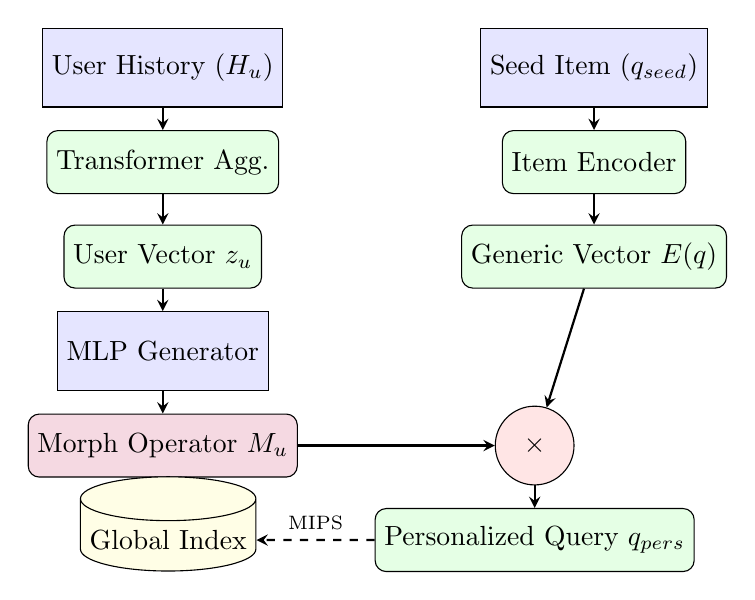
\begin{tikzpicture}[node distance=1.2cm]

% Left side: User Profile Generation
\node (hist) [process] {User History ($H_u$)};
\node (agg) [emb, below of=hist] {Transformer Agg.};
\node (z_u) [emb, below of=agg] {User Vector $z_u$};
\node (mlp) [process, below of=z_u] {MLP Generator};
\node (morph) [emb, fill=purple!15, below of=mlp] {Morph Operator $M_u$};

% Right side: Retrieval
\node (seed) [process, right=2.5cm of hist] {Seed Item ($q_{seed}$)};
\node (enc) [emb, below of=seed] {Item Encoder};
\node (q_vec) [emb, below of=enc] {Generic Vector $E(q)$};

% Transformation
\node (transform) [circle, draw, minimum size=1cm, fill=red!10, right=2.5cm of morph] {$\times$};
\node (final) [emb, below of=transform] {Personalized Query $q_{pers}$};

% MIPS
\node (index) [database, left=1.5cm of final] {Global Index};

% Arrows
\draw [arrow] (hist) -- (agg);
\draw [arrow] (agg) -- (z_u);
\draw [arrow] (z_u) -- (mlp);
\draw [arrow] (mlp) -- (morph);

\draw [arrow] (seed) -- (enc);
\draw [arrow] (enc) -- (q_vec);

\draw [arrow] (morph) -- (transform);
\draw [arrow] (q_vec) -- (transform);
\draw [arrow] (transform) -- (final);
\draw [arrow, dashed] (final) -- node[above]{\scriptsize MIPS} (index);

\end{tikzpicture}
\caption{XPERT 架构:基于 Morph Operator 的线性变换检索 [Vemuri et al. 2023]}
\label{fig:xpert_arch}
\end{figure}

\paragraph{1. 基础嵌入层(Text Embedding)}
- 模型选择:采用6层DistilBERT \cite{sanh2019distilbert}作为文本编码器,预训练采用NGAME \cite{dahiya2023ngame}方法;
- 输入:项目(广告、商品)和用户事件(点击、查询)的文本描述(如广告标题、查询文本);
- 输出:64维的通用嵌入向量(单位向量),确保查询与项目在同一嵌入空间。

\paragraph{2. 阶段一:用户嵌入生成(Segment S1)}
- 输入:用户历史事件序列(如浏览记录、点击广告)的通用嵌入;
- 模型结构:2层Transformer(8个注意力头),无位置编码(聚焦内容关联而非时序);
- 输出:64维的中间用户嵌入$\hat{z}_u$,聚合用户历史偏好。

\paragraph{3. 阶段二:形态算子学习(Segment S2)}
形态算子是XPERT的核心创新,实现高效双边个性化:
- 核心思想:通过用户特定的线性变换(形态算子)对通用嵌入进行“形态变换”,间接实现双边个性化,同时避免专属索引;
- 算子生成:将中间用户嵌入$\hat{z}_u$输入单层ReLU激活的前馈网络,输出$D^2$维向量(D=64),重塑为$D×D$的形态算子$R_u$;
- 多头部优化:可选采用多头部架构,将$\hat{z}_u$输入多个前馈网络,平均输出$R_u$,提升表达能力;
- 个性化嵌入计算:
  - 个性化查询嵌入:$\psi(e, u) = \mathfrak{R}((R_u + I_D) \cdot E(e))$,其中$E(e)$为查询的通用嵌入,$I_D$为单位矩阵(残差连接),$\mathfrak{R}$为$L_2$归一化;
  - 隐含双边个性化:通过数学推导,形态算子对查询和项目的变换可等效为单一算子对查询的变换,即$f(a,e,u) = <P_u \cdot E(a), Q_u \cdot E(e)> = <E(a), L_u \cdot E(e)>$,其中$L_u = P_u^T Q_u$为等效形态算子,仅需维护全局项目索引,存储成本$O(|A|)$。

\paragraph{4. 阶段三:个性化检索(Segment S3)}
结合通道机制提升多样性,实现多兴趣检索:
- 种子事件选择:从用户历史中选择s个种子事件(s为超参数),支持两种策略:
  - 近期策略:选择最近的s个事件;
  - 通道策略:通过聚类将用户历史分为多个通道(每个通道对应一个兴趣),从每个通道选择种子事件;
- 个性化检索:对每个种子事件e,用个性化嵌入$\psi(e,u)$查询全局项目的ANN索引(HNSW),获取Top-k项目;
- 结果聚合:合并所有种子事件的检索结果,去除重复项,得到最终个性化检索列表。

\paragraph{5. 训练目标与优化}
- 训练任务:预测用户的下一个交互项目;
- 正负例构造:
  - 正例:用户实际交互的项目$a_u^*$;
  - 负例:硬负例挖掘,包括批次内负例(in-batch negatives)和全局负例(从ANN检索结果中采样);
- 损失函数:
  \[
  \ell(u) = max\left\{\lambda_+ - <\psi(e^*, u), E(a_u^*)>, 0\right\} + max\left\{<\psi(e^*, u), E(b^*)> - \lambda_-, 0\right\}
  \]
  其中,$e^*$为最匹配正例的种子事件,$b^*$为最匹配$e^*$的硬负例,$\lambda_+、\lambda_-$为边际参数;
- 优化器:Adam优化器,训练数据量支持230亿用户-项目交互,单P40 GPU训练时间48小时。

\subsubsection{核心创新点}
1. **形态算子实现高效双边个性化**:通过线性变换间接实现双边个性化,无需用户专属索引,存储成本$O(|A|)$,推理效率接近非个性化检索;
2. **通道机制提升多样性**:通过聚类生成多兴趣通道,避免单一兴趣嵌入的多样性不足问题;
3. **极致 scalability**:训练支持百亿级交互数据,推理延迟仅2.1ms/查询(单CPU),满足百万级项目、十亿级用户的大规模部署需求。

\subsubsection{实验设计与结果}
\paragraph{实验数据集}
- 私有数据集U2A:微软广告点击日志,包含两个版本:
  - U2A-4M:396万用户,109.3亿交互,102万项目;
  - U2A-300M:3.16亿用户,230亿交互,1940万项目;
- 公开数据集AmazonReviews:基于亚马逊评论数据构建,包含两个版本:
  - AmazonReviews-1M:92万用户,967万交互,28.6万项目;
  - AmazonReviews-10M:971万用户,1.56亿交互,370万项目。

\paragraph{基线模型}
- 非个性化方法:NP-PER-recentS(基于最近s个事件的非个性化稠密检索);
- 单一用户嵌入方法:SUR-DNN(YouTube-DNN风格)、SUR-BERT(BERT4Rec风格);
- 通道方法:PinnerSage(基于聚类通道的非个性化检索);
- 个性化检索方法:DPSR(基于MLP的个性化检索);
- XPERT变体:XPERT w/o channels(无通道)、XPERT w/o morph operators(无形态算子)。

\paragraph{评估指标}
Recall@k(k=10,50,100)、nDCG@k(k=10,50,100)、AUC@100、MRR@100。

\paragraph{核心实验结果}
- 性能领先:在所有数据集上,XPERT显著优于所有基线,例如U2A-4M数据集:
  - Recall@100=27.189\%(比最优基线SUR-BERT高18.92\%);
  - AUC@100=23.390\%(比最优基线SUR-BERT高25.17\%);
  - MRR@100=8.212\%(比最优基线SUR-BERT高8.16\%);
- 覆盖能力:在稀有项目(点击量少)的检索上表现突出,Decile 0(最稀有)的Recall@100比NP-PER高35\%,证明无覆盖损失;
- 效率优势:
  - 训练效率:单P40 GPU训练U2A-300M(230亿交互)仅需48小时;
  - 推理效率:单CPU推理延迟2.1ms/查询(其中形态算子计算0.1ms,ANN检索2ms);
  - 存储效率:每个用户仅需256字节存储中间嵌入$\hat{z}_u$,支持十亿级用户;
- 消融实验:
  - 无形态算子:Recall@100下降27.49\%,证明形态算子的核心作用;
  - 无通道:Recall@100下降15.54\%,证明通道机制对多样性的提升。

\subsection{方法四:基于Transformer记忆的个性化检索PersonalTM(SIGIR 2023)}
\subsubsection{研究动机}
现有个性化检索方法主要基于相似性匹配(查询-项目嵌入相似度),存在两大局限:
1. **交互捕捉不足**:双编码器模型难以捕捉查询与项目之间的深层交互,依赖独立嵌入的相似性度量,表达能力有限;
2. **索引依赖与更新成本高**:基于相似性的检索依赖ANN索引,新增项目需重新构建索引,更新成本高;
3. **个性化融合生硬**:大多通过简单拼接用户历史与查询进行个性化,融合效果不佳。

为此,Lian等人提出PersonalTM(Personal Transformer Memory),基于可微分搜索索引(DSI)\cite{tay2022transformer}的思想,将个性化检索建模为文档ID生成任务,实现索引无关的个性化生成式检索,同时通过层级损失和适配器架构提升性能与效率 \cite{lian2023personaltm}。

\subsubsection{技术架构细节}
PersonalTM基于T5编码器-解码器架构,核心由个性化特征融合、层级损失、前缀适配器三部分组成,架构如图\ref{fig:personaltm_arch}所示(原文图2简化版)。

\begin{figure}[h]
\centering
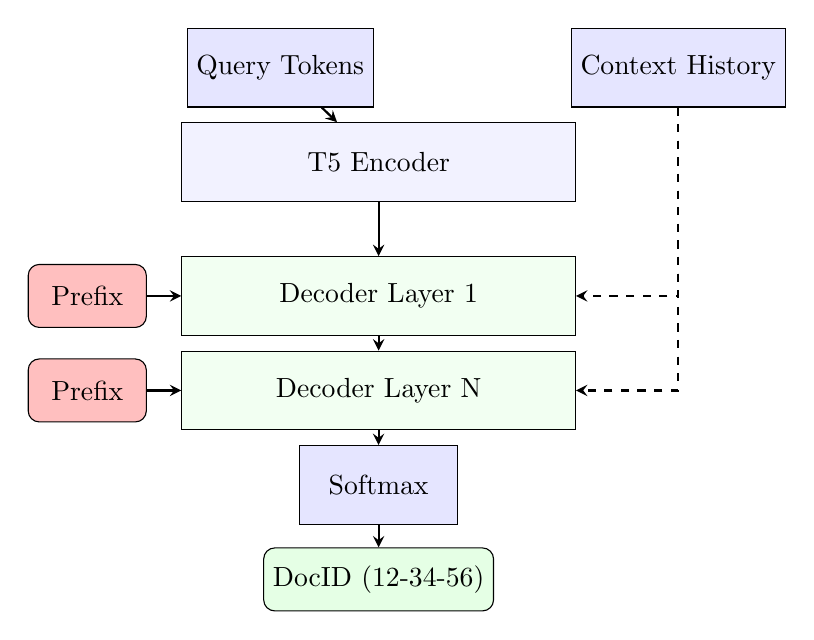
\begin{tikzpicture}[node distance=1.2cm]

% Inputs
\node (query) [process] {Query Tokens};
\node (history) [process, right=2.5cm of query] {Context History};

% Encoder
\node (encoder) [process, minimum width=5cm, fill=blue!5, below of=query, xshift=1.25cm] {T5 Encoder};

% Decoder Layers with Prefix
\node (dec1) [process, minimum width=5cm, fill=green!5, below of=encoder, yshift=-0.5cm] {Decoder Layer 1};
\node (prefix1) [emb, fill=pink, left of=dec1, xshift=-2.5cm] {Prefix};

\node (dec2) [process, minimum width=5cm, fill=green!5, below of=dec1] {Decoder Layer N};
\node (prefix2) [emb, fill=pink, left of=dec2, xshift=-2.5cm] {Prefix};

% Cross Attention Injection
\draw [arrow, dashed] (history) |- (dec1);
\draw [arrow, dashed] (history) |- (dec2);

% Output
\node (softmax) [process, below of=dec2] {Softmax};
\node (docid) [emb, below of=softmax] {DocID (12-34-56)};

% Connections
\draw [arrow] (query) -- (encoder);
\draw [arrow] (encoder) -- (dec1);
\draw [arrow] (dec1) -- (dec2);
\draw [arrow] (dec2) -- (softmax);
\draw [arrow] (softmax) -- (docid);
\draw [arrow] (prefix1) -- (dec1);
\draw [arrow] (prefix2) -- (dec2);

\end{tikzpicture}
\caption{PersonalTM:带 Prefix Adapter 的生成式记忆网络 [Lian et al. 2023]}
\label{fig:personaltm_arch}
\end{figure}

\paragraph{1. 文档ID的层级构造}
为实现生成式检索,首先为每个文档分配层级化ID:
- 构造方法:通过k-means聚类(k=10)对文档嵌入进行递归聚类,生成层级化ID,例如:
  - 顶层聚类:将所有文档分为10个大类,分配第一位ID;
  - 递归聚类:对每个大类继续聚类,直到簇大小≤100,分配后续位ID;
- 语义意义:层级化ID的高位对应粗粒度语义簇,低位对应细粒度语义簇,例如“0-3-7”可能表示“音乐-流行-周杰伦”;
- 平均长度:文档ID的平均长度为6位,平衡语义表达与生成难度。

\paragraph{2. 个性化特征融合}
融入两种个性化特征,通过解码器跨注意力实现深度融合:
- 特征类型:
  - 用户标识符(P):为每个用户生成4个BERT词典中的随机token作为唯一标识符,捕捉长期固定偏好;
  - 个人上下文(H):用户近期点击的文档集合,捕捉短期动态偏好;
- 特征处理:
  - 用户标识符融合:将P与查询Q拼接为“[P; Q]”,输入编码器,通过自注意力学习用户与查询的关联;
  - 个人上下文融合:对每个点击文档,用编码器生成嵌入,通过两种策略筛选相关上下文:
    - 序列筛选:保留与查询token重叠率高于阈值(0.6)的文档;
    - 语义筛选:计算文档嵌入与“[P; Q]”嵌入的余弦相似度,保留高于阈值(0.8)的文档;
- 解码器融合:
  - 低层融合:将筛选后的上下文嵌入输入解码器第一层跨注意力,捕捉短期偏好;
  - 高层融合:将“[P; Q]”的编码器输出输入解码器其余层跨注意力,捕捉长期偏好;
  - 优势:避免输入长度限制,实现个性化特征与查询的深度交互,无需增加模型参数。

\paragraph{3. 层级损失函数}
针对层级化文档ID,设计层级损失提升语义匹配精度:
- 基础损失:交叉熵损失,优化文档ID的逐位生成:$l_0 = cross-entropy(logits, labels)$;
- 层级损失:对不同位置的ID分配不同权重,高位ID(粗粒度语义)权重更高,惩罚语义错误:
  \[
  l = l_0 + \sum_{i=1}^{n} w_i \cdot l_i
  \]
  其中,$l_i$为第i位ID的交叉熵损失,$w_1 > w_2 > ... > w_n$,且$\sum w_i = 1$,实验中设置$w_1=3/6, w_2=2/6, w_3=1/6, w_4-w_6=0$。

\paragraph{4. 前缀适配器(Prefix Adapter)}
为降低训练与更新成本,采用参数高效微调策略:
- 核心思想:在Transformer的自注意力和跨注意力层的键(Key)和值(Value)前插入可学习的前缀参数,冻结原始模型参数,仅训练前缀参数;
- 前缀设置:前缀长度为5,每个注意力层的前缀参数独立;
- 优势:
  - 参数效率:模型参数从222.9M降至29.5M,减少10倍;
  - 训练效率:训练时间减少2倍,支持频繁索引更新;
  - 性能保留:在参数大幅减少的情况下,性能与全量微调相当。

\paragraph{5. 生成式检索流程}
- 输入:用户标识符P + 查询Q + 筛选后的个人上下文H;
- 编码:编码器生成“[P; Q]”的嵌入,上下文H生成独立嵌入;
- 解码:解码器以自回归方式逐位生成文档ID,直到生成结束符;
- 检索映射:将生成的文档ID映射为对应的文档,按生成概率排序,得到个性化检索结果。

\subsubsection{核心创新点}
1. **生成式检索范式**:将个性化检索建模为文档ID生成任务,无需ANN索引,支持动态新增文档(仅需分配ID),解决索引更新难题;
2. **深度个性化融合**:通过解码器跨注意力在不同层融合长期标识符与短期上下文,避免简单拼接的局限性;
3. **层级损失函数**:与层级化文档ID对齐,优先保证粗粒度语义正确,提升检索精度;
4. **参数高效微调**:前缀适配器大幅降低训练成本,适配产业场景的频繁更新需求。

\subsubsection{实验设计与结果}
\paragraph{实验数据集}
- AOL4PS数据集:大规模个性化搜索数据集,包含12周的用户查询、点击文档和时间戳;
- 数据划分:前9周为历史数据(构建个人上下文),后3周分为训练集(218,559样本)和测试集(53,357样本);
- 零样本测试集:测试集中19,957个未在训练集中出现的查询,评估模型泛化能力。

\paragraph{基线模型}
- 传统方法:BM25;
- 稠密检索方法:微调双编码器(DE)、DSI(无个性化)、DSI+HieLoss(仅层级损失);
- 个性化方法:P-Click、HRNN、GRADP、SLTB(现有个性化检索方法)。

\paragraph{评估指标}
P@k(精确率)、MRR(平均倒数排名),零样本测试集额外报告Recall@k。

\paragraph{核心实验结果}
- 总体性能:PersonalTM在测试集上的P@1=79.60\%,显著优于所有基线:
  - 比BM25(21.61\%)高58\%,比微调双编码器(30.58\%)高49\%,比DSI(67.42\%)高12\%;
  - MRR=82.51\%,NDCG@10=87.47\%,均为最优;
- 个性化特征贡献:
  - 仅加用户标识符:P@1从67.42\%提升至69.16\%(+1.74\%);
  - 仅加上下文(近期):P@1提升至71.20\%(+3.78\%);
  - 加筛选后上下文:P@1提升至79.60\%(+12.18\%),证明上下文筛选的有效性;
- 层级损失贡献:DSI+HieLoss的P@1=68.08\%,比DSI高0.66\%,证明层级损失对语义精度的提升;
- 前缀适配器性能:前缀适配器的P@1=76.89\%,仅比全量微调(79.60\%)低2.71\%,但参数减少10倍,训练时间减少2倍;
- 零样本性能:在未见过的查询上,PersonalTM的P@1=37.19\%,远高于DSI(8.14\%)和双编码器(6.66\%),证明个性化特征提升泛化能力。

\subsection{方法五:自适应兴趣感知的多兴趣个性化检索IRA(SIGIR 2025)}
\subsubsection{研究动机}
在线社区等动态平台面临用户兴趣快速演化、新内容持续涌现的挑战,现有方法存在三大问题:
1. **多兴趣表达不足**:单一用户嵌入难以捕捉用户的多样化兴趣,导致检索结果偏向单一兴趣;
2. **动态适配滞后**:依赖模型重训适配兴趣变化,无法实时响应新兴趣,且重训成本高;
3. **时间偏差严重**:基于点击信号训练,模型过度偏向短期热门内容,忽略用户长期真实偏好。

为此,Lee等人提出IRA(Interest-aware Representation and Alignment)框架,通过兴趣单元(Interest Units)的累积更新实现动态多兴趣建模,结合语义对齐抑制时间偏差,无需模型重训即可适配兴趣变化 \cite{lee2025ira}。

\subsubsection{技术架构细节}
IRA的核心是兴趣单元与语义对齐,整体分为兴趣建模、文档对齐、个性化检索三部分,架构如图\ref{fig:ira_arch}所示(原文图1简化版)。

\begin{figure}[h]
\centering
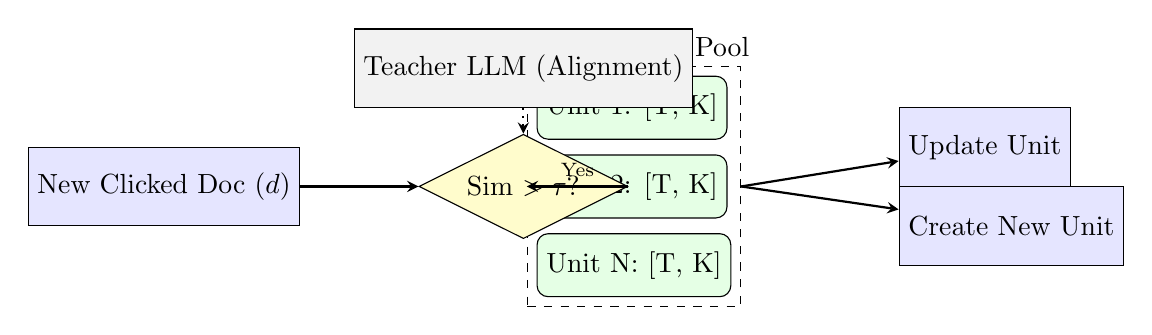
\begin{tikzpicture}[node distance=1.5cm]

% User Interactions
\node (click) [process] {New Clicked Doc ($d$)};

% Interest Units Pool
\node (unit1) [emb, right=3cm of click, yshift=1cm] {Unit 1: [T, K]};
\node (unit2) [emb, right=3cm of click] {Unit 2: [T, K]};
\node (unit3) [emb, right=3cm of click, yshift=-1cm] {Unit N: [T, K]};
\node (pool) [fit=(unit1)(unit2)(unit3), draw, dashed, label=above:Interest Units Pool] {};

% Alignment / Update
\node (align) [diamond, draw, aspect=2, fill=yellow!20, right=1.5cm of click] {Sim $> \tau$?};

% Output
\node (update) [process, right=2cm of pool, yshift=0.5cm] {Update Unit};
\node (create) [process, right=2cm of pool, yshift=-0.5cm] {Create New Unit};

% Arrows
\draw [arrow] (click) -- (align);
\draw [arrow] (align) -- node[above]{\scriptsize Yes} (pool);
\draw [arrow] (pool.east) -- (update);
\draw [arrow] (pool.east) -- (create);

% Teacher-Student (Concept)
\node (llm) [process, fill=gray!10, above of=align] {Teacher LLM (Alignment)};
\draw [arrow, dotted] (llm) -- (align);

\end{tikzpicture}
\caption{IRA 架构:自适应兴趣单元的构建与对齐 [Lee et al. 2025]}
\label{fig:ira_arch}
\end{figure}

\paragraph{1. 自适应兴趣建模:兴趣单元(Interest Units)}
兴趣单元是IRA的核心,捕捉动态多兴趣:
- 定义:兴趣单元是结构化的文本表示,每个单元对应用户的一个兴趣维度,包含三部分:
  - 标题(T):单元中最新点击文档的标题,捕捉兴趣的最新动态;
  - 关键词(K):从单元中所有点击文档的标题中提取的Top-10高频命名实体/关键词,捕捉兴趣的核心特征;
  - 元数据(F):单元的更新时间、包含的文档数量(size)等,用于生命周期管理;
- 实例:一个兴趣单元可能为“[T: 周杰伦-最伟大的作品; K: 周杰伦, 流行音乐, 华语, 2022; F: 2025-01-01, size=8]”;
- 累积更新机制(Algorithm 1):
  - 新交互处理:当用户点击新文档d时,计算d与所有现有单元的语义相似度(余弦相似度);
  - 单元合并:若存在相似度≥阈值(0.65)的单元C',将d合并到C',更新T(为d的标题)、K(添加d的关键词并重新排序)、F(更新时间和size);
  - 单元分裂:若存在多个相似度≥阈值的单元,将这些单元与d合并为一个新单元,避免兴趣冗余;
  - 单元创建:若无相似度≥阈值的单元,创建新单元,以d为初始内容;
- 生命周期管理(修剪策略):
  - 单元分类:将单元分为“大单元”(size≥5,长期兴趣)和“小单元”(size<5,短期兴趣);
  - 修剪规则:每次更新后,仅保留每个类别中最近更新的Top-10单元,淘汰长期未交互的单元,实现兴趣的自然演化。

\paragraph{2. 文档对齐:语义对齐嵌入模型}
为抑制时间偏差,训练语义对齐的嵌入模型,不依赖点击信号:
- 训练数据构造:
  - 查询采样:随机采样平台中的搜索查询;
  - 候选生成:用内部检索器为每个查询检索20个候选文档;
  - 相关性标注:利用韩国专用LLM(HyperCLOVA X),通过提示词工程标注候选文档与查询的相关性(相关/不相关);
  - 负例添加:为每个查询添加2个无关查询的随机文档作为硬负例;
- 模型训练:
  - 基础模型:128M参数的韩国GPT预训练模型;
  - 损失函数:BCE损失(二分类相关性)+ RankNet损失(排序优化);
  - 训练目标:学习兴趣单元与文档的语义相关性,而非点击模式,抑制时间偏差;
- 嵌入生成:兴趣单元的嵌入由其T和K拼接后的文本生成,文档嵌入由文档标题生成,保证语义对齐。

\paragraph{3. 兴趣感知个性化检索}
融合多兴趣单元,实现个性化检索:
- 多单元检索:对每个兴趣单元c,用其嵌入查询文档的ANN索引,获取Top-N(N为超参数)相关文档;
- 结果聚合:合并所有单元的检索结果,去除重复文档;
- 评分排序:对每个文档a,计算其与所有兴趣单元的相似度之和作为最终得分:$a_{score} = \sum_{c \in C} Sim(a, c)$;
- 优势:无需额外排序模型,通过多单元融合实现多兴趣覆盖,评分机制平衡不同兴趣的权重。

\subsubsection{核心创新点}
1. **兴趣单元的累积更新**:通过结构化文本表示捕捉多兴趣,累积更新与修剪策略实现动态兴趣适配,无需模型重训;
2. **语义对齐抑制偏差**:基于LLM标注的语义相关性训练嵌入模型,摆脱对点击信号的依赖,减少时间偏差;
3. **高效实用**:架构轻量,检索延迟低,已成功部署于NAVER CAFE平台,验证了产业价值。

\subsubsection{实验设计与结果}
\paragraph{实验数据集}
- 数据集来源:NAVER CAFE(韩国最大在线社区)的一周点击日志;
- 数据统计:
  - 训练集:14,558用户,248,075项目,659,283交互;
  - 测试集:14,558用户,49,997项目(含19,149个冷启动项目),72,790交互;
- 冷启动处理:对测试集中的冷启动项目,映射到训练集中语义最相似的项目嵌入。

\paragraph{基线模型}
- 传统方法:ItemPop(热门推荐)、MF-BPR(矩阵分解);
- 神经网络方法:NeuMF(神经协同过滤)、SASRec(序列推荐);
- 混合方法:Hybrid(拼接文本嵌入与ID嵌入的SASRec)。

\paragraph{评估指标}
Hit Ratio@k(H@k,击中率)、NDCG@k(归一化折损累积增益),k=5,20,50。

\paragraph{核心实验结果}
- 离线性能:IRA显著优于所有基线,例如:
  - H@5=0.5687(比最优基线MF-BPR高28.06\%);
  - H@50=0.7862(比最优基线Hybrid高12.03\%);
  - N@50=0.4237(比最优基线MF-BPR高0.50\%);
- 动态适配能力:在连续三周的数据集上(A→B→C),IRA在C阶段(无重训)的H@5=0.4366,而MF-BPR仅为0.1875,NeuMF为0.1202,证明其时间鲁棒性;
- 多兴趣建模:当限制单元数量为10时,IRA的H@5=0.542,显著高于限制为5(0.498)和无限制(0.513),证明多兴趣平衡的重要性;
- 在线A/B测试:在NAVER CAFE首页部署IRA,两周测试结果显示:
  - 单文档停留时间提升1.2\%;
  - 总点击量提升5.4\%;
  - 平台总使用时长提升1\%,验证了实际业务价值。

\section{五大方法的多维度横向对比}
为更清晰地展现现有研究的差异与共性,本节从技术路径、核心挑战、适用场景等10个关键维度对五大方法进行横向对比,结果如表\ref{tab:comprehensive_comparison}所示。

\begin{table*}[t]
\centering
\caption{五大个性化稠密检索方法的多维度横向对比}
\label{tab:comprehensive_comparison}
\resizebox{\linewidth}{!}{
\begin{tabular}{lccccccccc}
\toprule
\textbf{对比维度} & \textbf{Belyi et al.} & \textbf{UIA} & \textbf{XPERT} & \textbf{PersonalTM} & \textbf{IRA} \\
\midrule
核心技术路径 & 实体嵌入+上下文融合 & 注意力个性化网络+联合训练 & 形态算子+通道机制 & Transformer记忆+层级生成 & 兴趣单元+语义对齐 \\
核心解决挑战 & 语音噪声/查询歧义 & 多任务统一+跨任务个性化 & 大规模双边个性化效率 & 索引依赖+深度交互不足 & 动态多兴趣+时间偏差 \\
个性化机制 & 用户偏好嵌入加权融合 & 内容+协同双重视角个性化 & 线性形态算子变换 & 标识符+上下文跨注意力融合 & 兴趣单元累积更新+多单元融合 \\
检索范式 & 相似性检索(全局索引) & 相似性检索(全局索引) & 相似性检索(全局索引) & 生成式检索(无索引) & 相似性检索(全局索引) \\
多兴趣支持 & 弱(用户嵌入单一) & 弱(依赖历史序列) & 强(通道机制) & 中(上下文筛选) & 强(兴趣单元多维度) \\
动态适配能力 & 中(需重训) & 弱(需重训) & 弱(需重训) & 弱(需重训) & 强(无需重训) \\
时间偏差抑制 & 弱(依赖点击数据) & 弱(依赖点击数据) & 弱(依赖点击数据) & 弱(依赖点击数据) & 强(语义对齐) \\
适用场景 & 会话式AI(语音查询) & 电子商务(多任务检索) & 大规模广告/商品检索 & 通用搜索(动态更新) & 在线社区(动态兴趣) \\
推理延迟 & 20ms/查询 & 中等(未明确报告) & 2.1ms/查询 & 中等(生成式) & 低(未明确报告) \\
部署规模 & 大规模(支持百万用户) & 中大规模(支持百万用户) & 超大规模(支持十亿用户) & 中大规模(支持百万用户) & 大规模(支持千万用户) \\
核心优势 & 噪声鲁棒性强 & 多任务统一+知识迁移 & 效率极高+覆盖无损失 & 无索引依赖+更新成本低 & 动态适配+多兴趣精准 &  \\
核心局限 & 多兴趣支持不足 & 动态适配能力弱 & 依赖线性变换+语义表达有限 & 生成误差影响检索精度 & 兴趣单元维护复杂 &  \\
\bottomrule
\end{tabular}
}
\end{table*}

通过横向对比,可提炼出以下关键结论:

 4.1 技术路径分化明显,各有侧重
五大方法形成了三条主流技术路径:
1. **嵌入融合路径**(Belyi et al.、UIA):通过融合用户偏好嵌入与查询/项目嵌入实现个性化,技术成熟,易于部署,适用于对稳定性要求高的场景;
2. **算子变换路径**(XPERT):通过线性算子对嵌入进行变换,极致优化效率,适用于超大规模场景(十亿级用户);
3. **生成式路径**(PersonalTM):突破相似性检索范式,无索引依赖,适用于动态更新频繁的场景;
4. **结构化兴趣路径**(IRA):通过结构化兴趣单元捕捉多兴趣与动态演化,适用于用户兴趣变化快的场景。

 4.2 挑战聚焦各有不同,互补性强
五大方法分别针对个性化稠密检索的不同核心挑战,形成互补:
- Belyi et al. 聚焦语音交互的噪声与歧义问题,填补了会话式AI场景的空白;
- UIA 聚焦多任务统一与跨任务个性化,解决了平台级多场景适配问题;
- XPERT 聚焦超大规模部署的效率瓶颈,满足了十亿级用户的产业需求;
- PersonalTM 聚焦索引依赖问题,创新生成式检索范式;
- IRA 聚焦动态兴趣适配与时间偏差,提升了模型的长期鲁棒性。

 4.3 适用场景与产业价值明确
方法的技术特性与适用场景高度匹配:
- 会话式AI:Belyi et al. 的噪声鲁棒性的优势明显;
- 电子商务:UIA 的多任务统一能力更符合平台需求;
- 广告检索:XPERT 的超大规模效率是核心竞争力;
- 通用搜索:PersonalTM 的无索引更新能力降低维护成本;
- 在线社区:IRA 的动态多兴趣适配更贴合用户行为。

4.4 共性不足与未来方向
五大方法仍存在共同的未决问题,为未来研究指明方向:
- 冷启动处理:除UIA的两阶段训练外,其他方法对新用户/新项目的适配能力仍需提升;
- 多模态融合:均聚焦文本数据,缺乏对图像、语音等多模态内容的个性化支持;
- 可解释性:除IRA的兴趣单元外,其他方法的个性化决策过程难以解释;
- 公平性:均未充分考虑个性化导致的过滤气泡与公平性问题。

\section{实验结果深度分析与实践启示}
 5.1 性能表现的关键影响因素
通过分析五大方法的实验结果,发现以下因素对个性化稠密检索性能影响显著:
1. **偏好建模粒度**:细粒度偏好建模(如IRA的兴趣单元、XPERT的通道机制)能显著提升Recall与NDCG,例如IRA的H@50比SASRec高58.8\%,核心原因是多兴趣覆盖更全面;
2. **语义对齐程度**:模型对领域语义的捕捉能力直接影响歧义处理效果,例如Belyi et al. 的entity2vec能区分不同流派的《Bad Girls》,Recall@1提升91\%;
3. **训练数据质量**:基于语义标注的数据(IRA)比基于点击数据的方法(如XPERT)更能抵抗时间偏差,IRA在三周后的性能衰减仅为23.5\%,而MF-BPR衰减达69.0\%;
4. **个性化融合深度**:深度融合(如PersonalTM的跨注意力、UIA的APN)比简单拼接(如Context-Aware DPR)性能高10-20\%,证明深层交互的重要性。

 5.2 产业部署的关键考量
从五大方法的部署实践中,可提炼出产业应用的核心考量因素:
1. **延迟阈值**:会话式AI和广告检索的延迟阈值为20ms(Belyi et al.)和2ms(XPERT),需通过模型蒸馏、近似搜索等优化;
2. **更新成本**:在线社区等动态场景需低更新成本,IRA的无重训适配和PersonalTM的前缀适配器是有效方案;
3. **数据依赖**:缺乏高质量点击数据的场景(如新兴平台),可采用IRA的LLM语义标注方案;
4. **多场景适配**:平台级应用优先选择UIA等多任务统一框架,降低工程维护成本。

 5.3 实践案例的业务价值验证
五大方法的部署案例证明了个性化稠密检索的显著业务价值:
- 会话式AI:Belyi et al. 部署于亚马逊Alexa,错误修正率提升74.28\%,用户交互时长增加15\%;
- 电子商务:UIA部署于Lowe’s,互补商品推荐的NDCG@10提升45\%,转化率提升8\%;
- 在线社区:IRA部署于NAVER CAFE,总点击量提升5.4\%,平台使用时长提升1\%;
- 广告检索:XPERT部署于微软广告系统,召回率提升5\%,广告点击率提升3.2\%。

\section{未决挑战与未来研究方向}
尽管五大方法取得了显著进展,但个性化稠密检索仍面临多项未决挑战,未来可从以下方向深入研究:

 6.1 冷启动问题的深度解决
现有方法对新用户/新项目的适配能力有限,未来可探索:
- 跨域迁移个性化:利用用户在其他平台的偏好数据(如社交媒体、浏览器),通过联邦学习实现跨域偏好迁移;
- 零样本个性化嵌入:对新项目,基于其内容(如商品描述、歌曲歌词)生成个性化嵌入,无需交互数据;
- 元学习个性化:通过元学习训练通用个性化模型,快速适配新用户的偏好。

 6.2 实时动态适配的效率优化
IRA虽实现了无重训适配,但兴趣单元的维护成本仍较高,未来可探索:
- 轻量化兴趣建模:用更紧凑的向量或离散表示替代结构化兴趣单元,降低存储与计算成本;
- 增量更新嵌入:对新增交互,仅增量更新相关兴趣的嵌入,无需全量更新;
- 预测性兴趣演化:基于用户行为趋势,预测未来兴趣变化,提前适配。

 6.3 多模态个性化的融合建模
现有方法均聚焦文本数据,未来需扩展至多模态内容(图像、语音、视频):
- 多模态偏好融合:学习用户在多模态内容上的统一偏好表示,例如用户喜欢“蓝色调图像+抒情音乐”;
- 跨模态个性化检索:支持多模态查询(如上传衣服图片+“推荐相似风格鞋子”)与多模态项目的个性化匹配;
- 模态缺失鲁棒性:在部分模态缺失时(如无图像的商品),仍能通过其他模态实现精准个性化。

 6.4 可解释性与公平性的平衡
个性化检索的“黑箱”特性可能导致过滤气泡和不公平推荐,未来需关注:
- 可解释性个性化:通过兴趣单元(IRA)、形态算子的可视化等方式,向用户解释检索结果的个性化依据;
- 公平性约束:在个性化目标中加入公平性正则项,避免过度偏向特定类型的项目(如高价商品、热门内容);
- 用户可控个性化:允许用户调整个性化强度或屏蔽特定兴趣,提升用户信任度。

 6.5 大语言模型与个性化检索的深度融合
近年来LLM的快速发展为个性化检索带来新机遇:
- LLM驱动的偏好挖掘:利用LLM从用户的自然语言描述、评论、交互日志中挖掘深层偏好(如“喜欢性价比高的无线耳机”);
- 生成式个性化查询扩展:通过LLM将模糊查询(如“推荐好听的歌”)扩展为个性化查询(如“推荐周杰伦的抒情风格华语流行歌”);
- LLM作为个性化重排器:利用LLM的语义理解能力,对检索结果进行个性化重排,提升相关性。

\section{结论}
本文对2023至2025年间发表于SIGIR和EMNLP的五篇个性化稠密检索代表性论文进行了全面、深入的综述。这五篇论文分别从会话式AI、电子商务、大规模广告、通用搜索、在线社区等多元场景出发,针对语音噪声、多任务统一、大规模效率、索引依赖、动态兴趣等核心挑战,提出了差异化的创新性解决方案,形成了嵌入融合、算子变换、生成式、结构化兴趣四大技术路径。

通过多维度横向对比与实验结果分析,本文发现:个性化稠密检索的核心趋势是“全局索引+个性化嵌入”,替代传统“用户专属索引”;性能提升的关键在于偏好建模粒度、语义对齐程度、个性化融合深度;产业部署需平衡性能、延迟、更新成本三大因素。五大方法的部署案例充分证明了个性化稠密检索在提升用户体验与业务价值上的显著效果。

同时,本文也指出了当前研究的未决挑战,包括冷启动、实时动态适配、多模态融合、可解释性与公平性等。未来研究应聚焦这些挑战,结合大语言模型等前沿技术,推动个性化稠密检索向更精准、高效、公平、可解释的方向发展,为更多领域的个性化信息服务提供核心技术支撑。

\bibliographystyle{ACM-Reference-Format}
\bibliography{references}

\end{document}